\documentclass[11pt,a4paper]{article}
\usepackage[margin=2.5cm]{geometry}
\usepackage{amsmath,amssymb}
\usepackage{booktabs,tabularx}
\usepackage{enumitem}
\usepackage{graphicx}
\usepackage{float}
\usepackage{xcolor}
\usepackage[most]{tcolorbox}
\usepackage[round,authoryear]{natbib}
\usepackage[colorlinks=true,linkcolor=blue!50!black,citecolor=blue!50!black]{hyperref}

\definecolor{boxbg}{HTML}{EEF3F8}
\definecolor{askbg}{HTML}{FFF1E0}
\definecolor{okbg}{HTML}{E6F4E7}
\definecolor{cardframe}{HTML}{2F6FAE}
\newcommand{\ask}[1]{\par\smallskip\noindent\colorbox{askbg}{\parbox{\dimexpr\linewidth-2\fboxsep}{\textbf{Your decisions.} #1}}\par\smallskip}
\newcolumntype{Y}{>{\raggedright\arraybackslash}X}

% One card per measure, always with the same rows in the same order.
\newtcolorbox{card}[1]{enhanced, breakable, colback=white, colframe=cardframe,
  boxrule=0.6pt, arc=2pt, left=6pt, right=6pt, top=4pt, bottom=4pt,
  title={#1}, fonttitle=\bfseries, coltitle=white}
\newcommand{\row}[1]{\par\smallskip\noindent\textbf{#1}\enspace}

\title{Proposal, version 3\\[2pt]\large A simpler way to score a run (\texttt{sec:pf:measures})}
\author{For review before anything is applied}
\date{5 October 2026}

\begin{document}
\sloppy
\maketitle

\noindent Version 2 tried to repair the current scoring section one
problem at a time. Version 3 replaces the scoring itself with a smaller
scheme taken from the lifelong MAPD literature. Version 2 is kept as
\texttt{scoring\_proposal\_v2.pdf} in the same folder. Nothing in the thesis
has been changed, and the figures are drafts in \texttt{scoring\_proposal/}.

\tableofcontents

%----------------------------------------------------------------
\section{Why change the scoring}
\label{sec:why}

\paragraph{The main test cannot be computed.} The research question is
formalised in \texttt{eq:rqformal} as a comparison of $\mathcal{J}$ under
adaptive and fixed storage. $\mathcal{J}$ adds five quantities with
weights $q_{\mathrm{svc}}$, $q_{\mathrm{mov}}$, $q_{\mathrm{wait}}$,
$q_{\mathrm{conc}}$ and $q_{\mathrm{back}}$. No chapter gives these
weights a value, and the Method's parameter tables do not list them even
as TBD. The central result therefore rests on five numbers that do not
exist.

\paragraph{Any choice of weights would be arbitrary.} The section keeps
runtime out of $\mathcal{J}$ because seconds cannot be traded against
timesteps. The same holds inside $\mathcal{J}$. Service time is in
timesteps, movement cost in cost units, backlog in tasks, and
concentration is a fraction. Each weight sets an exchange rate between two
units that the thesis would have to defend.

\paragraph{Lifelong MAPD scores with much less.} The paper that defines
lifelong MAPD, \citet{ma2017lifelong_mapf}, judges an algorithm by one
number, the service time. It accepts a run only if the service time stays
bounded, and reports runtime per timestep next to it.
Section~\ref{sec:sources} lists what each paper in
\texttt{thesis-progress/papers/} measures.

\paragraph{Throughput and backlog answer one question.} Tasks arrive at a
fixed rate $\lambda_{\mathrm{task}}$. While the fleet keeps up, it finishes
tasks as fast as they arrive, so throughput equals the arrival rate and the
backlog stays small. Throughput and backlog only depart from that when the
fleet falls behind. Together they answer whether the fleet keeps up. They
are not two separate scores.

%----------------------------------------------------------------
\section{The principles behind the new scheme}
\label{sec:principles}

\begin{enumerate}[leftmargin=1.5em]
  \item \textbf{One primary result.} Mean service time decides whether
    adaptive storage beats fixed storage. No weighted sum is used.
  \item \textbf{Every other measure answers a named question.} Each one
    either checks that a run is valid or explains why the primary result
    changed. None of them is traded against service time.
  \item \textbf{Borrowed measures are cited and not claimed.} A measure
    taken from a paper is used as that paper defines it, with the
    citation, and is not presented as a contribution of the thesis. Where
    the thesis adapts a measure, the change is stated, and only the change
    is the thesis's own responsibility. A measure with no source in the
    literature is marked as the thesis's own.
  \item \textbf{Each measure has the same layout.} The question it
    answers, one sentence saying what it counts, the formula, a worked
    number, its source, and its role.
  \item \textbf{Every worked number comes from the same two examples.}
    These are the timeline of tasks $\tau_1$ to $\tau_4$
    (Figure~\ref{fig:timeline}) and the warehouse with agents $a_1$ to
    $a_4$ (Figure~\ref{fig:share}), both drawn on bases the thesis already
    uses.
\end{enumerate}

%----------------------------------------------------------------
\section{The four questions}
\label{sec:questions}

A run is scored by four questions, asked in this order.\par\medskip
\noindent\begin{tabularx}{\linewidth}{@{}lYl@{}}
  \toprule
  Question & Measure & Role \\
  \midrule
  1. Does the fleet keep up? & throughput against arrival rate, backlog & check \\
  2. How fast is a task served? & mean service time $\bar\zeta_T$ & \textbf{primary result} \\
  3. Why did it change? & blocked time, crowding, traffic share, movement cost & explanation \\
  4. What does deciding cost? & runtime per timestep $\kappa_T$ & reported \\
  \bottomrule
\end{tabularx}

\begin{figure}[H]
  \centering
  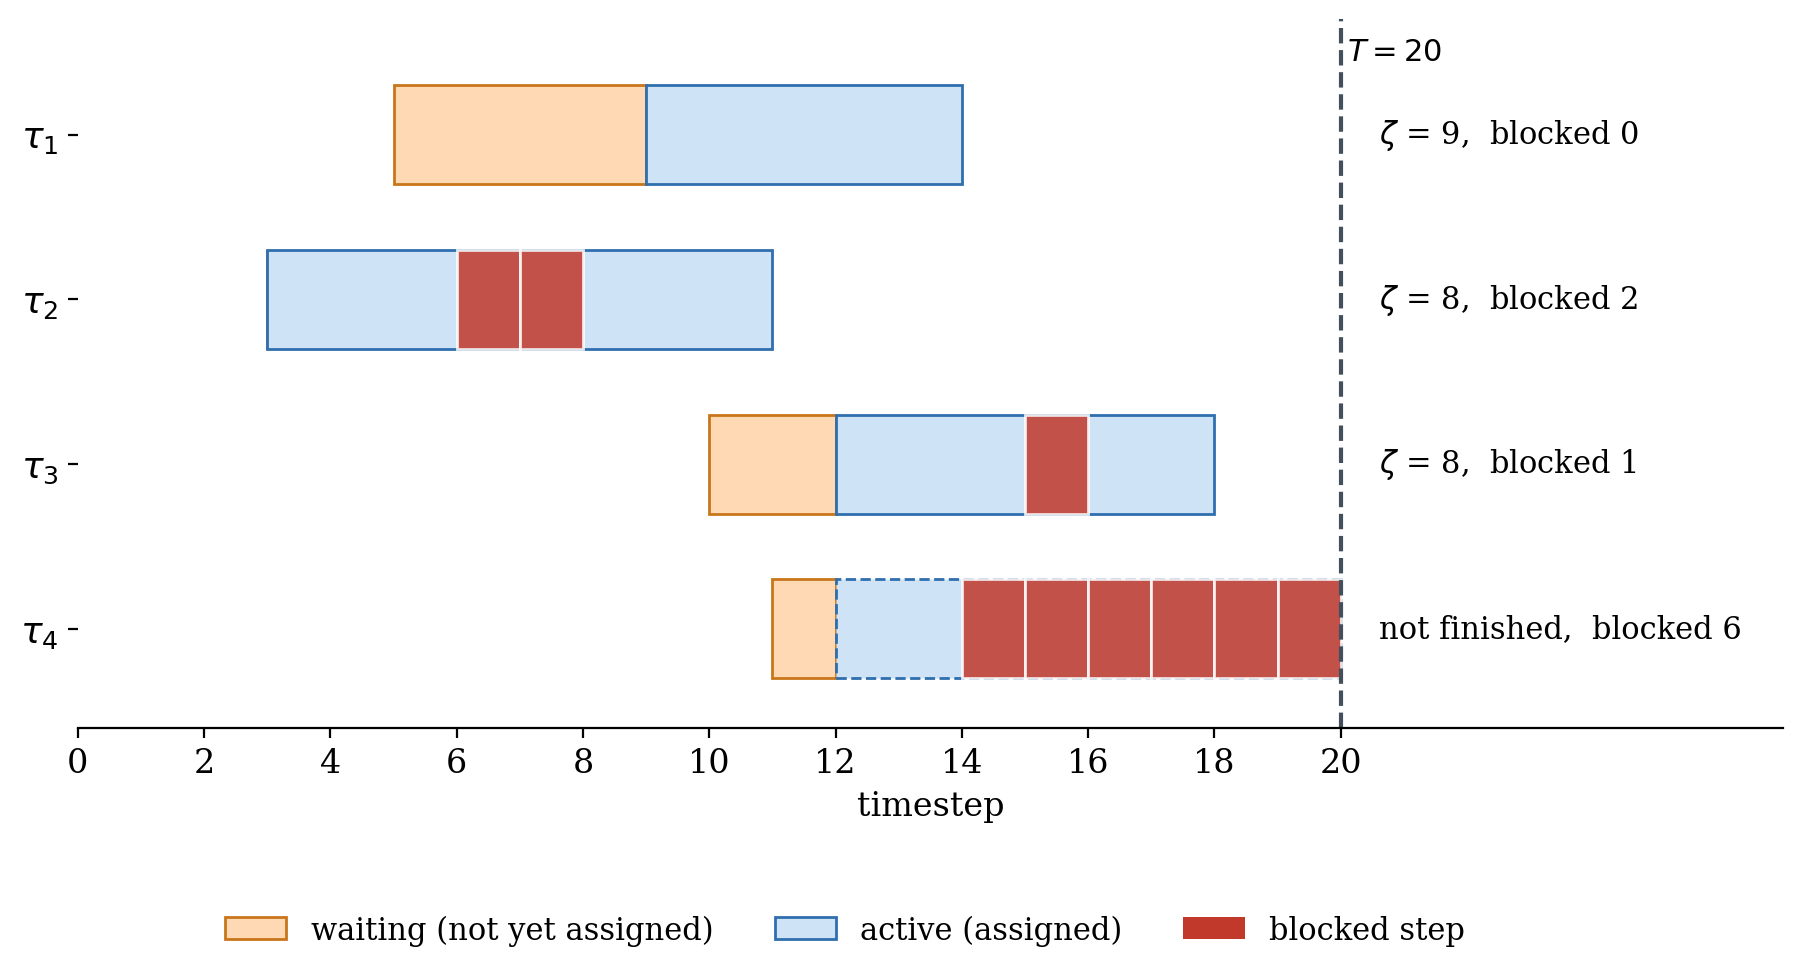
\includegraphics[width=0.85\linewidth]{timeline_stuck_draft.png}
  \caption{Four tasks over a horizon $T=20$. $\tau_4$ is stuck from $t=14$
  and never finishes. This is the worked example for questions 1 to 3.}
  \label{fig:timeline}
\end{figure}

%----------------------------------------------------------------
\subsection{Question 1. Does the fleet keep up?}

\begin{card}{Throughput against arrival rate, and backlog}
\row{Question.} Is the fleet finishing tasks as fast as they arrive?

\row{What it counts.} Throughput is the number of tasks finished per
timestep. The fleet keeps up when throughput stays close to the rate at
which tasks arrive. The backlog, the number of tasks released but not yet
finished, is logged at every timestep and plotted, so a run that falls
behind can be seen.

\row{Formula.}
\[
  \Lambda_T = \frac{|\mathcal{C}_T|}{T}, \qquad
  \text{the run keeps up if } \Lambda_T \ge f_{\mathrm{up}}\,\lambda_{\mathrm{task}},
  \qquad B_t = |\mathcal{Q}_t| + |\mathcal{B}_t| .
\]

\row{Worked number.} In Figure~\ref{fig:timeline}, four tasks are
released and three finish within $T=20$. Throughput is $3/20 = 0.15$ per
timestep against $4/20 = 0.20$ released, a ratio of $0.75$. The backlog
ends at $B_{20} = 1$, the stuck task $\tau_4$. Without $\tau_4$ the ratio
would be $1$ and the backlog $0$.

\row{Source.} \citet{ma2017lifelong_mapf} count a lifelong MAPD instance
as solved only if the service time of all tasks stays bounded, which is
the same as keeping up. Throughput as completed tasks per unit time is the
pick rate that \citet{krnjaic2022warehouse_marl} optimise. \emph{Own
part:} the ratio test and its threshold $f_{\mathrm{up}}$.

\row{Role.} A check, applied before anything else. A run that does not
keep up is reported as such, and its service time is not compared,
because service time only counts finished tasks.
\end{card}

%----------------------------------------------------------------
\subsection{Question 2. How fast is a task served?}

\begin{card}{Mean service time $\bar\zeta_T$, the primary result}
\row{Question.} On average, how long does a task take from its release to
its delivery?

\row{What it counts.} For each finished task, the number of timesteps
between its release and its delivery, averaged over the finished tasks.
The wait before assignment counts too, because the order is waiting during
that time as well (\texttt{fig:lifecycle}).

\row{Formula.}
\[
  \bar\zeta_T = \frac{1}{|\mathcal{C}_T|}\sum_{\tau_j\in\mathcal{C}_T}\zeta_j,
  \qquad \zeta_j = t_j^{\mathrm{finish}} - t_j^{\mathrm{released}}
  \quad (\texttt{eq:servicetime}).
\]

\row{Worked number.} $\tau_1$, $\tau_2$ and $\tau_3$ take $9$, $8$ and $8$
timesteps, so $\bar\zeta_T = 25/3 \approx 8.33$.

\row{Source.} \citet{ma2017lifelong_mapf} define the service time as ``the
average number of timesteps \ldots\ needed to finish executing each task
after it was added to the task set'' and use it to evaluate a MAPD
algorithm. The thesis uses it unchanged. \emph{Own part:} none.

\row{Role.} The primary result. Adaptive storage beats fixed storage under
a controller $\pi$ when both runs keep up and $\bar\zeta_T$ is lower by
more than the variation between seeds (Section~\ref{sec:formal}).
\end{card}

%----------------------------------------------------------------
\subsection{Question 3. Why did the result change?}

These four measures explain a change in service time. They are reported
next to it and never added to it.

\begin{card}{Blocked time $W_T$}
\row{Question.} How much time do agents lose standing still once they have
a task?

\row{What it counts.} From assignment to delivery, every timestep in which
the task's agent does not move, either because it chose to wait or
because conflict resolution turned its move into a wait. The count is
averaged over the finished tasks, like service time.

\row{Formula.}
\[
  W_T = \frac{1}{|\mathcal{C}_T|}\sum_{\tau_j\in\mathcal{C}_T}
        \sum_{t=t_j^{\mathrm{assigned}}}^{t_j^{\mathrm{finish}}-1}\omega_j(t)
  \qquad (\texttt{eq:waiting}, \text{ unchanged}).
\]

\row{Worked number.} $\tau_1$, $\tau_2$ and $\tau_3$ are blocked $0$, $2$
and $1$ times, so $W_T = 3/3 = 1$. The stuck task $\tau_4$ is not counted
here, because question 1 already catches it.

\row{Source.} No paper in the folder reports blocked time. \emph{Own
part:} the whole measure. It is built from the override flag of the
conflict-resolution operator, which the Method already logs.

\row{Role.} Explains service time, and answers the waiting part of RQ3.
\end{card}

\begin{card}{Crowding $\bar\delta_T$}
\row{Question.} How crowded was the space around the agents?

\row{What it counts.} Each agent's congestion feature $\delta_i(t)$, the
share of its field of view taken by other agents, averaged over every
agent and every timestep.

\row{Formula.}
\[
  \bar\delta_T = \frac{1}{mT}\sum_{t=0}^{T-1}\sum_{i=1}^{m}\delta_i(t)
  \qquad (\delta_i(t) \text{ from \texttt{eq:congestion}}).
\]

\row{Worked number.} At $t=11$ in \texttt{observation.png}, $a_1$ reads
$\delta_1 = 2/5 = 0.4$. If the four agents read $0.4$, $0.2$, $0.4$ and
$0.2$ throughout, then $\bar\delta_T = 0.3$. On average, 30\% of the space
around an agent was taken.

\row{Source.} The per-agent density is the one CRAMP
\citep{pham2024optimizingcrowdawaremultiagentpath} computes, the agents in
the field of view divided by the free space there. CRAMP uses it only
inside its reward. \emph{Own part:} averaging it into a reported outcome.

\row{Role.} Explains blocked time. Crowding without blocking costs
nothing, as with a convoy that never stops. Blocking without crowding
points to the controller rather than to the traffic. Answers the
congestion part of RQ3.
\end{card}

\begin{card}{Traffic share of the busiest edges $\Gamma_T$}
\row{Question.} Does the traffic pile up on a few aisles?

\row{What it counts.} The share of all edge traversals that falls on the
busiest 10\% of the edges. If traffic is spread evenly, the busiest 10\%
of edges carry about 10\% of it. The higher the share, the more the
traffic piles up.

\row{Formula.} With $\mu_T(e)$ the traversals of edge $e$ over the horizon
and $E_{10}$ the $\lceil 0.1\,|E|\rceil$ edges with the largest
$\mu_T(e)$,
\[
  \Gamma_T = \frac{\sum_{e\in E_{10}}\mu_T(e)}{\sum_{e\in E}\mu_T(e)} .
\]

\row{Worked number.} The warehouse has 36 edges, so the busiest 4 count.
In Figure~\ref{fig:share}, each panel has 72 traversals and the busiest 4
edges carry 8, 24 and 36 of them, so $\Gamma_T$ is $11\%$, $33\%$ and
$50\%$.

\row{Source.} No paper in the folder reports traffic concentration.
\emph{Own part:} the whole measure. It replaces the entropy $H_T$ and the
index $C_T$. Every edge always counts, used or not, so the corridor
problem of Decision~A in version~2 does not arise.

\row{Role.} Answers the concentration part of RQ3, the risk that feedback
between storage and routing funnels traffic onto a few aisles.
\end{card}

\begin{figure}[H]
  \centering
  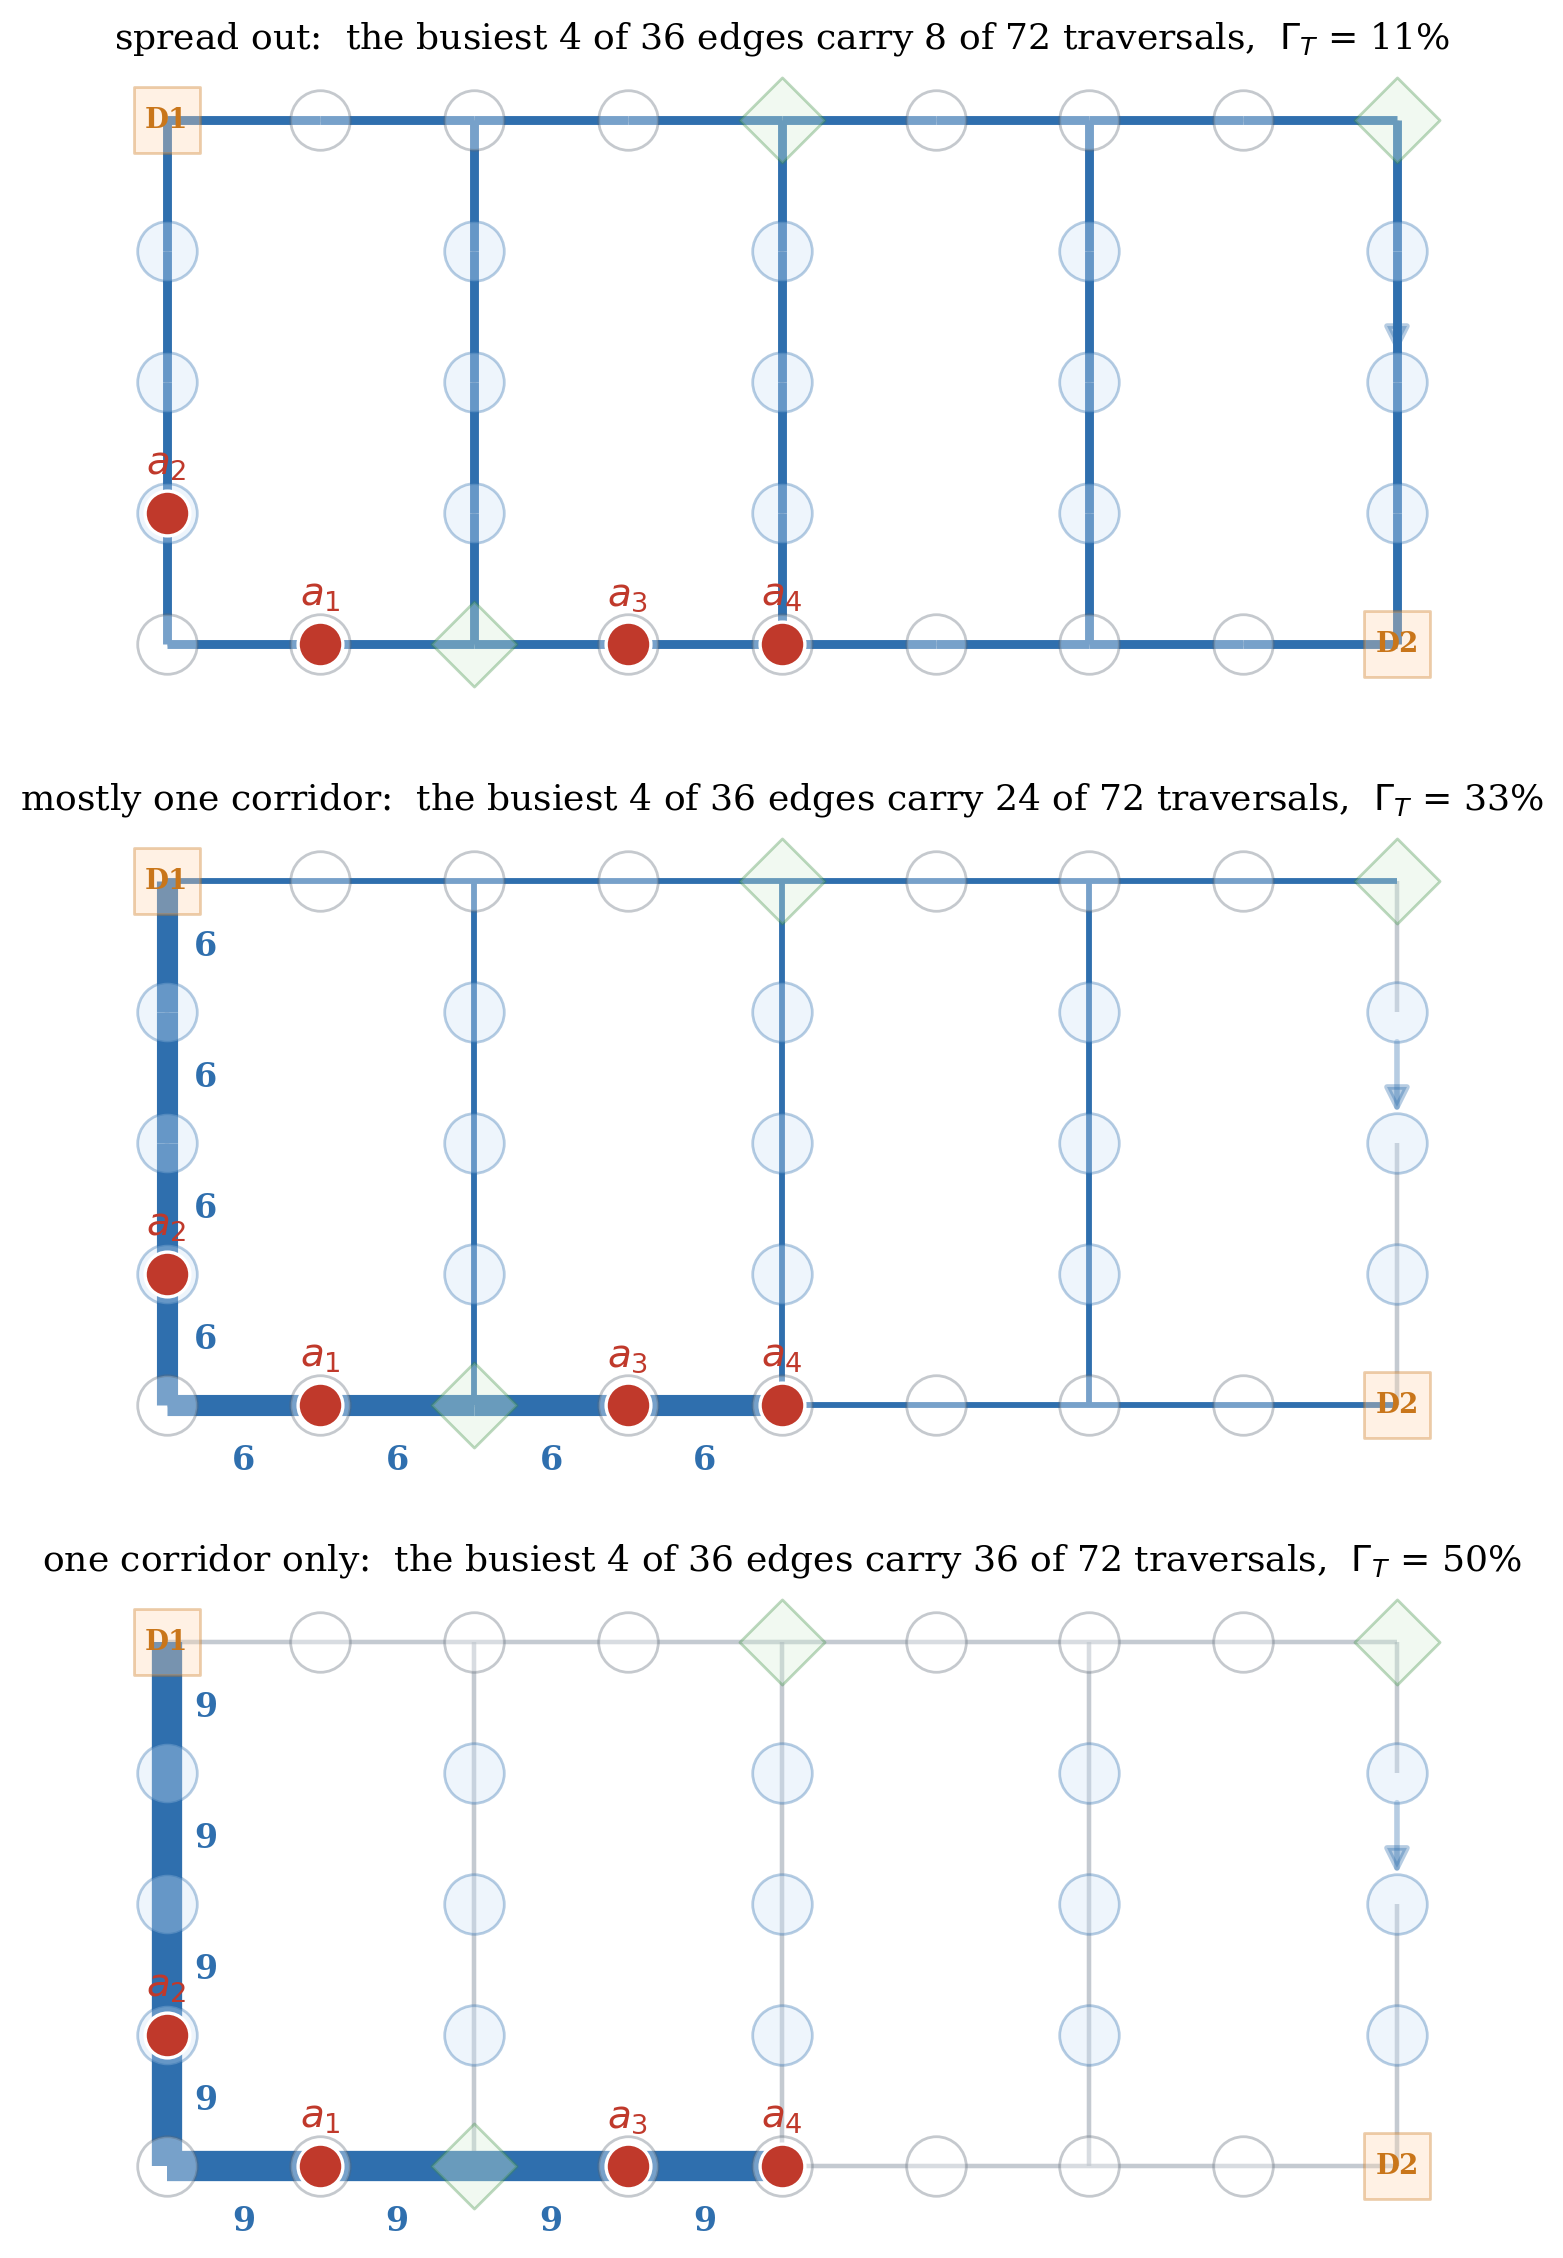
\includegraphics[width=0.66\linewidth]{concentration_share_draft.png}
  \caption{The concentration figure scored by the share of the busiest 4 of
  36 edges, on the warehouse and agents of \texttt{observation.png}.}
  \label{fig:share}
\end{figure}

\begin{card}{Movement cost per finished task $\bar c_T$}
\row{Question.} How much effort does one delivered task take?

\row{What it counts.} The one-step cost $\hat c$ of every agent at every
timestep, summed and divided by the number of finished tasks. Standing
still costs $c_{\mathrm{wait}}$, so it counts too (E1 from version~2).

\row{Formula.}
\[
  \bar c_T = \frac{1}{|\mathcal{C}_T|}\sum_{i=1}^{m}\sum_{t=0}^{T-1}
             \hat c\bigl(\ell_i(t),\ell_i(t+1)\bigr)
  \qquad (\texttt{eq:movementcost}, \text{ unchanged}).
\]

\row{Worked number.} If the four agents make 72 moves of cost 1, wait 8
times at $c_{\mathrm{wait}} = 0.5$ and finish 12 tasks, then
$\bar c_T = (72 + 4)/12 \approx 6.33$. These cost values only serve the
example.

\row{Source.} CRAMP reports ``total moves'', the number of non-idle
actions of all agents \citep{pham2024optimizingcrowdawaremultiagentpath}.
\emph{Own part:} weighting each step by its cost, since edges in this
graph differ in length, and dividing by the finished tasks, since a
lifelong run has no fixed number of tasks.

\row{Role.} Answers the movement cost part of RQ1. Adaptive storage can
shorten trips, and this is where it shows.
\end{card}

%----------------------------------------------------------------
\subsection{Question 4. What does deciding cost?}

\begin{card}{Runtime per timestep $\kappa_T$}
\row{Question.} How long does the controller take to choose the next joint
action?

\row{What it counts.} The wall-clock time of assignment and routing
together at each timestep, averaged over the horizon. How it is measured
is fixed in \texttt{sec:impl:cost}.

\row{Formula.}
\[
  \kappa_T = \frac{1}{T}\sum_{t=0}^{T-1}\kappa(t)
  \qquad (\texttt{eq:runtime}, \text{ unchanged}).
\]

\row{Worked number.} If deciding takes $2$\,ms at every timestep,
$\kappa_T = 2$\,ms.

\row{Source.} \citet{ma2017lifelong_mapf} report runtime per timestep for
every algorithm and ask for it to stay below one second for real-time
lifelong operation. \emph{Own part:} none.

\row{Role.} Reported. It is in seconds, so it is never compared with
service time.
\end{card}

%----------------------------------------------------------------
\section{The research question, formally}
\label{sec:formal}

The decision problem becomes one sentence. Choose the storage rule and the
controller with the shortest expected service time among those that keep
up. Formally,
\[
  (F^\star,\pi^\star) \in \arg\min_{F\in\mathcal{F},\,\pi\in\Pi}
  \mathbb{E}\bigl[\bar\zeta_T(F,\pi)\bigr]
  \quad\text{subject to keeping up and the constraints of the model.}
\]
The expectation is over the order stream and the random seeds. The study
estimates it by the mean over evaluation seeds.

The thesis does not solve this problem. It compares fixed and adaptive
storage under each controller, so \texttt{eq:rqformal} reads
\[
  \mathbb{E}\bigl[\bar\zeta_T(F,\pi)\bigr] <
  \mathbb{E}\bigl[\bar\zeta_T(F_{\mathrm{fix}},\pi)\bigr]
  \quad\text{by a margin exceeding seed variation, with both runs keeping up.}
\]

\paragraph{Robustness.} The main RQ also asks about robustness. Under this
scheme it needs no extra measure. A gain is robust if it holds in most
seeds and keeps its sign as the load grows (RQ4). \citet{lau2022mapd}
report each measure as a mean with its standard error over five seeds,
which is the reporting style proposed here. The example from version~2
still applies. A larger mean gain that loses in two of five seeds is less
robust than a smaller gain that wins in all five.

%----------------------------------------------------------------
\section{What the literature measures}
\label{sec:sources}

All papers below are in \texttt{thesis-progress/papers/} and already in
\texttt{references.bib}. The table lists what each one reports and what
the thesis takes from it.

\medskip
\noindent\begin{tabularx}{\linewidth}{@{}p{0.2\linewidth}YY@{}}
  \toprule
  Paper & What it reports & Used here \\
  \midrule
  \citet{ma2017lifelong_mapf}, lifelong MAPD
    & service time as the measure of an algorithm, bounded service time as
      the condition for solving an instance, makespan, runtime per timestep
    & service time (Q2), the keep-up condition (Q1), runtime (Q4).
      Makespan is not used, see below. \\
  \citet{krnjaic2022warehouse_marl}, warehouse MARL
    & pick rate, completed order-lines per hour, as the single objective
    & throughput (Q1), and the case for one objective \\
  \citet{lau2022mapd}, MAPD with MAPF and MARL
    & flow time and makespan for the first delivery, reward, deliveries
      per agent, episode time, as means with standard errors over five
      seeds. The paper notes that MAPF and MARL use different measures,
      which makes the two hard to compare.
    & the reporting over seeds (robustness) \\
  CRAMP \citep{pham2024optimizingcrowdawaremultiagentpath}
    & success rate, makespan, total moves, collision count. Crowd density
      is used in the reward only.
    & the per-agent density (crowding, Q3), total moves as the origin of
      movement cost (Q3) \\
  PICO \citep{li2022pico}, PRIMAL \citep{sartoretti2019primal},
  \citet{vanKnippenberg2021}
    & success rate, makespan, collisions, share of solved instances
    & none, see below \\
  \bottomrule
\end{tabularx}

\paragraph{Measures not used, and why.}
\begin{itemize}[nosep]
  \item \emph{Makespan and success rate} are one-shot MAPF measures. Every
    agent has one goal, and the run ends when all have arrived. A lifelong
    run has no moment when everything is done, so the keep-up check takes
    the place of success.
  \item \emph{Collision count} is always zero here, because conflict
    resolution prevents every collision by construction. The cost of the
    prevented collisions shows up in blocked time instead.
  \item \emph{Flow time for the first delivery} looks only at the first
    task of each agent, which in a lifelong run says little about the
    steady pattern the study compares.
\end{itemize}

%----------------------------------------------------------------
\section{What is removed and what it touches}
\label{sec:touches}

\paragraph{Removed from the model.}
\begin{itemize}[nosep]
  \item $\mathcal{J}(F,\pi)$ (\texttt{eq:functional}) and its five weights
    $q_\bullet$.
  \item The entropy $H_T$, the index $C_T$, $E^{+}_T$ and $p_T(e)$
    (\texttt{eq:entropy}, \texttt{eq:concentration}), with the
    \texttt{[G8]} convention for a single used edge.
  \item The backlog as a weighted term. The backlog stays, as part of the
    keep-up check.
\end{itemize}

\paragraph{Added.} $\Gamma_T$, $\bar\delta_T$ and the threshold
$f_{\mathrm{up}}$. The letter $\Gamma$ is unused in the notation table,
although lower-case $\gamma$ is the discount factor. If that is too close,
another letter is easy to pick.

\paragraph{Places in the thesis that change.}
\begin{itemize}[nosep]
  \item The scoring section itself, rewritten as the four questions.
  \item \texttt{eq:decisionproblem} and \texttt{eq:rqformal}, as in
    Section~\ref{sec:formal}.
  \item The Project Description's list of dependent variables.
  \item The scope paragraph on deadlines (\texttt{[K2]}), which says a late
    delivery degrades $\mathcal{J}$ and that deadlines could become a term
    in \texttt{eq:functional}. It would refer to service time instead.
  \item The opening of the Method chapter, which names $\mathcal{J}$ as a
    framing device.
  \item The instrumentation section, where $H_T$ becomes $\Gamma_T$.
  \item The notation table, for the rows above.
  \item One new \texttt{[Axx]} tag and a \texttt{GAPS.md} entry recording
    the change and its reasons.
\end{itemize}

\paragraph{Not touched.} The RL reward was already defined apart from
$\mathcal{J}$, as a tool for good behaviour, so training does not change.
The storage rule $F$ and its objective do not change either.

%----------------------------------------------------------------
\section{What happens to the version 2 decisions}

\begin{center}
\begin{tabular}{lp{0.58\linewidth}}
  \toprule
  Version 2 item & In version 3 \\
  \midrule
  A. Normalising the entropy & No longer needed, because $\Gamma_T$ counts every edge. \\
  B. Crowding $\bar\delta_T$ & Kept, in question 3. \\
  C. Robustness & Seed spread and load, Section~\ref{sec:formal}. \\
  D. Stuck tasks & Settled. They fail the keep-up check in question 1. \\
  E. Name ``movement cost'' & Kept, with the clause on $c_{\mathrm{wait}}$. \\
  New structure & Replaced by the four questions, in the same spirit,
    with a plain overview first. \\
  Timeline figure & Kept, and now the main worked example. \\
  New concentration figure & Kept, scored by $\Gamma_T$. \\
  Fixes P1 to P11 & P1, P2, P3, P9, P10 and P11 still apply. P4, P5 and
    P7 are settled by the new scheme. P6 and P8 are covered by the new
    list of dependent variables and the movement cost card. \\
  \bottomrule
\end{tabular}
\end{center}

%----------------------------------------------------------------
\section{Your decisions}

\ask{\begin{enumerate}[nosep,leftmargin=1.2em]
  \item Replace $\mathcal{J}$ with the four questions, with service time
    as the one primary result?
  \item The keep-up test is throughput of at least $f_{\mathrm{up}}$ times
    the arrival rate. Should $f_{\mathrm{up}}$ stay TBD in the Method
    tables, or do you have a value in mind?
  \item The busiest 10\% of edges for $\Gamma_T$, or another share?
  \item Should the thesis state in one sentence which measures are
    borrowed and which are its own, as the cards do here?
\end{enumerate}}

\noindent Once you agree, the changes are applied as listed in
Section~\ref{sec:touches}. The figure scripts then move to
\texttt{thesis-progress/scripts/images/}, with outputs copied to both
\texttt{Images/} folders, and nothing is committed before you have read
the result.

\bibliographystyle{plainnat}
\bibliography{../thesis/references}

\end{document}
